\chapter{Results} \label{app:results}
\section{Experiment 1: Feasibility} % =============================================================================

\section{Experiment 2: 3D Context} % ==============================================================================

\begin{sidewaystable}[htbp]
   \centering
   \caption[Segmentation Evaluation Metrics for the different Architectures]{}
   \begin{tabular}{l*{6}{l}}
      \toprule
      Cohort	& Neural Network	& DICE				& VS				& AVD				& HD95				& HD				\\
      			&					&					&					& (mm)				& (mm)				& (mm)				\\
      \midrule
      Patient   & FCNN\_2D\_Base  & $0.704 \pm 0.139$ & $0.882 \pm 0.098$ & $2.880 \pm 2.671$ & $16.526 \pm 17.025$ & $63.696 \pm 20.903$ \\
                & FCNN\_3D\_3to1  & $0.749 \pm 0.139$ & $0.896 \pm 0.123$ & $\mathbf{1.979 \pm 2.190}$ & $\mathbf{10.807 \pm 13.393}$ & $\mathbf{56.262 \pm 23.958}$ \\
                & FCNN\_3D\_5to1  & $\mathbf{0.765 \pm 0.123}$ & $\mathbf{0.898 \pm 0.110}$ & $2.001 \pm 2.401$ & $12.418 \pm 19.104$ & $56.304 \pm 28.746$ \\
                & FCNN\_3D\_5to3  & $0.717 \pm 0.135$ & $0.883 \pm 0.105$ & $2.995 \pm 3.148$ & $19.312 \pm 22.545$ & $65.740 \pm 22.811$ \\
                & FCNN\_3D\_Proj  & $0.712 \pm 0.136$ & $0.889 \pm 0.094$ & $3.119 \pm 3.038$ & $19.878 \pm 21.613$ & $60.762 \pm 22.985$ \\
                & FCNN\_3D\_Patch & $0.682 \pm 0.128$ & $0.876 \pm 0.101$ & $3.581 \pm 2.724$ & $24.241 \pm 20.896$ & $70.737 \pm 26.853$ \\                
      \midrule
      Volunteer & FCNN\_2D\_Base  & $0.861 \pm 0.057$ & $0.921 \pm 0.056$ & $0.643 \pm 0.866$ & $1.644  \pm 2.321 $ & $\mathbf{35.380 \pm 32.720}$ \\
                & FCNN\_3D\_3to1  & $0.860 \pm 0.073$ & $0.925 \pm 0.043$ & $0.734 \pm 0.859$ & $2.260  \pm 2.336 $ & $39.327 \pm 29.429$ \\
                & FCNN\_3D\_5to1  & $\mathbf{0.878 \pm 0.048}$ & $\mathbf{0.928 \pm 0.048}$ & $ 0.509 \pm 0.393	$ & $1.537  \pm 1.784 $ & $46.515 \pm 30.853$ \\
                & FCNN\_3D\_5to3  & $0.855 \pm 0.052$ & $0.928 \pm 0.062$ & $\mathbf{0.473 \pm 0.435}$ & $\mathbf{1.350  \pm 1.365} $ & $39.033 \pm 30.589$ \\                
                & FCNN\_3D\_Proj  & $0.842 \pm 0.051$ & $0.917 \pm 0.067$ & $0.861 \pm 0.813$ & $1.642  \pm 1.549 $ & $40.584 \pm 30.139$ \\
                & FCNN\_3D\_Patch & $0.806 \pm 0.068$ & $0.888 \pm 0.085$ & $1.166 \pm 1.164$ & $7.992  \pm 13.474$ & $39.796 \pm 27.201$ \\
      \bottomrule
   \end{tabular}
   \label{tab:results_3d_context}
\end{sidewaystable}

\begin{figure}[htbp]
	\centering
	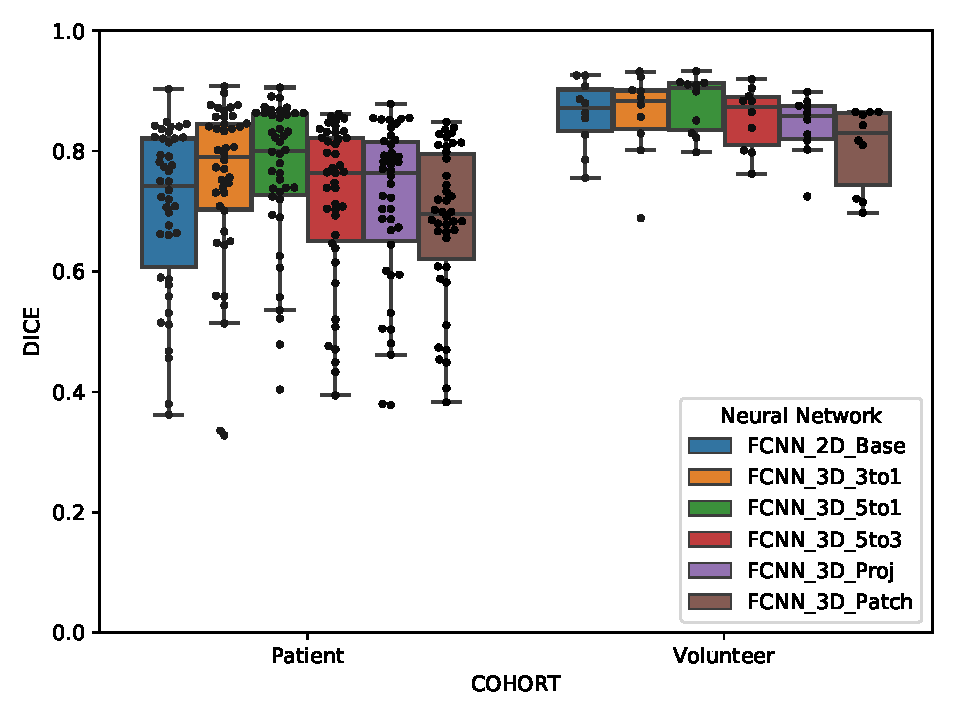
\includegraphics[width=0.8\textwidth]{boxplot_DICE}
    \caption[Boxplot for the \acrlong{dice}.]{Boxplot for the \acrlong{dice}.}
    \label{fig:results_boxplot_dice}
\end{figure}
\begin{figure}[htbp]
	\centering
	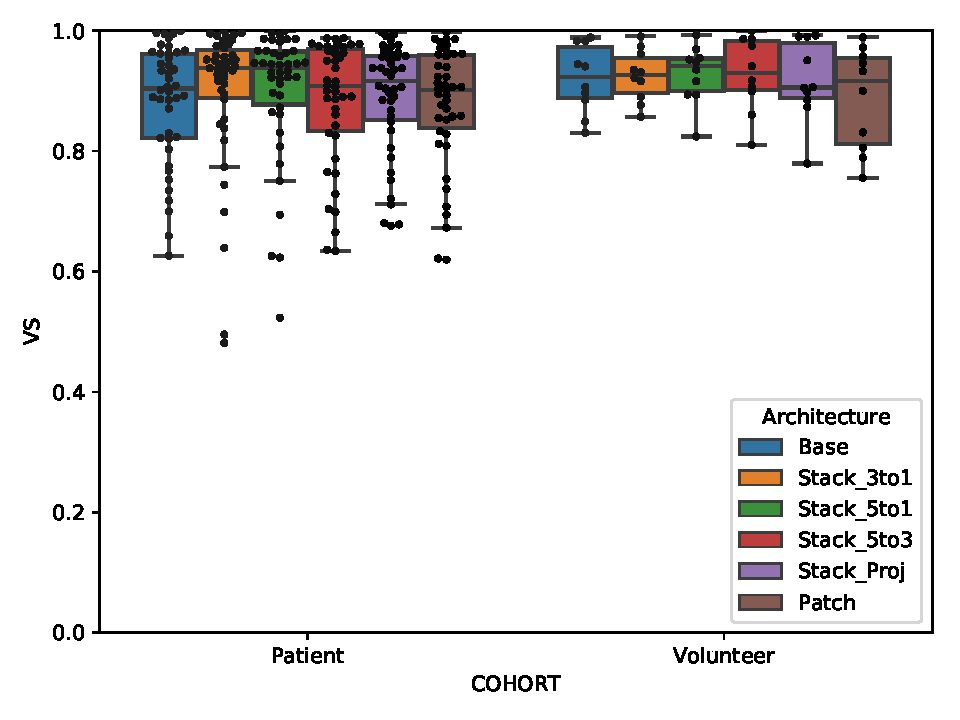
\includegraphics[width=0.8\textwidth]{boxplot_VS}
    \caption[Boxplot for the \acrlong{vs}.]{Boxplot for the \acrlong{vs}.}
    \label{fig:results_boxplot_vs}
\end{figure}
\begin{figure}[htbp]
	\centering
	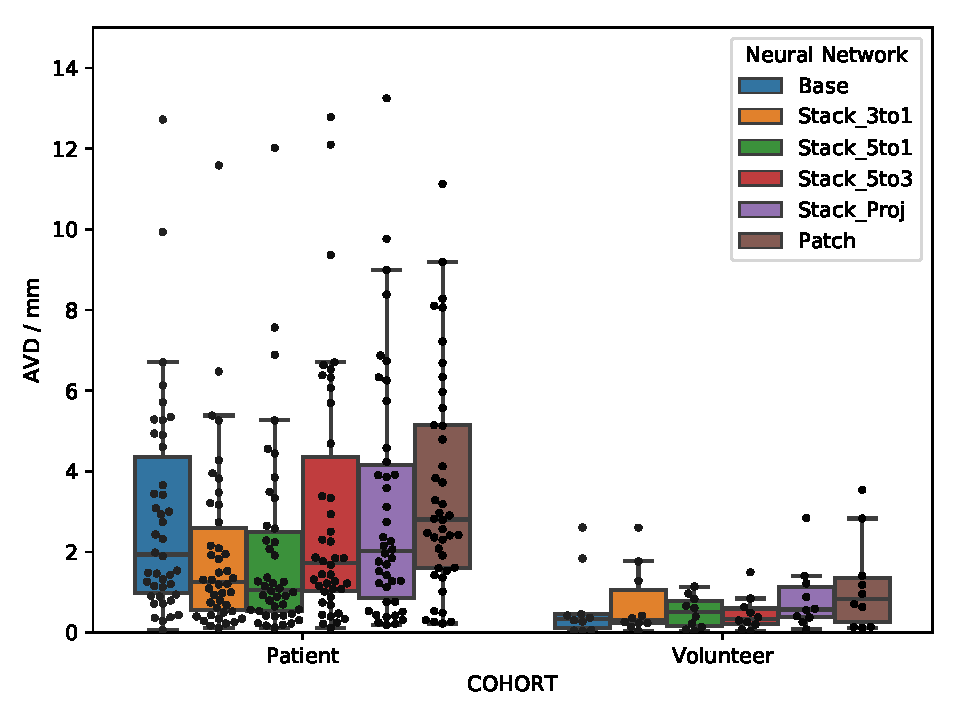
\includegraphics[width=0.8\textwidth]{boxplot_AVD}
    \caption[Boxplot for the \acrlong{avd}.]{Boxplot for the \acrlong{avd}.}
    \label{fig:results_boxplot_avd}
\end{figure}
\begin{figure}[htbp]	
	\centering
	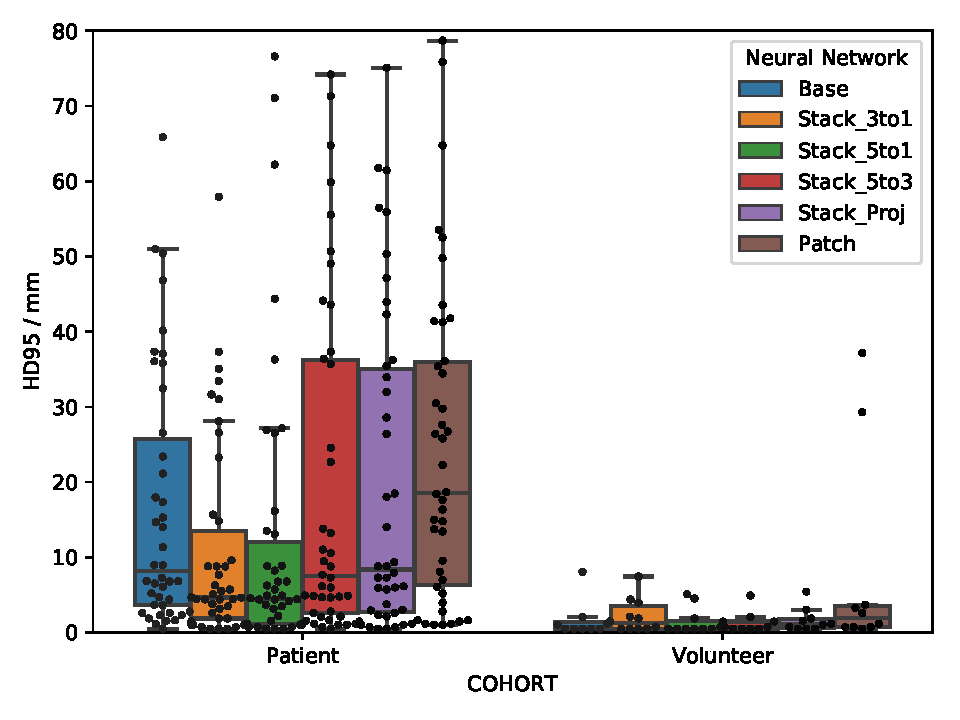
\includegraphics[width=0.8\textwidth]{boxplot_HD95}
    \caption[Boxplot for the 95\textsuperscript{th} percentile \acrlong{hd}.]{Boxplot for the 95\textsuperscript{th} percentile \acrlong{hd}.}
    \label{fig:results_boxplot_hd95}
\end{figure}
\begin{figure}[htbp]	
	\centering
	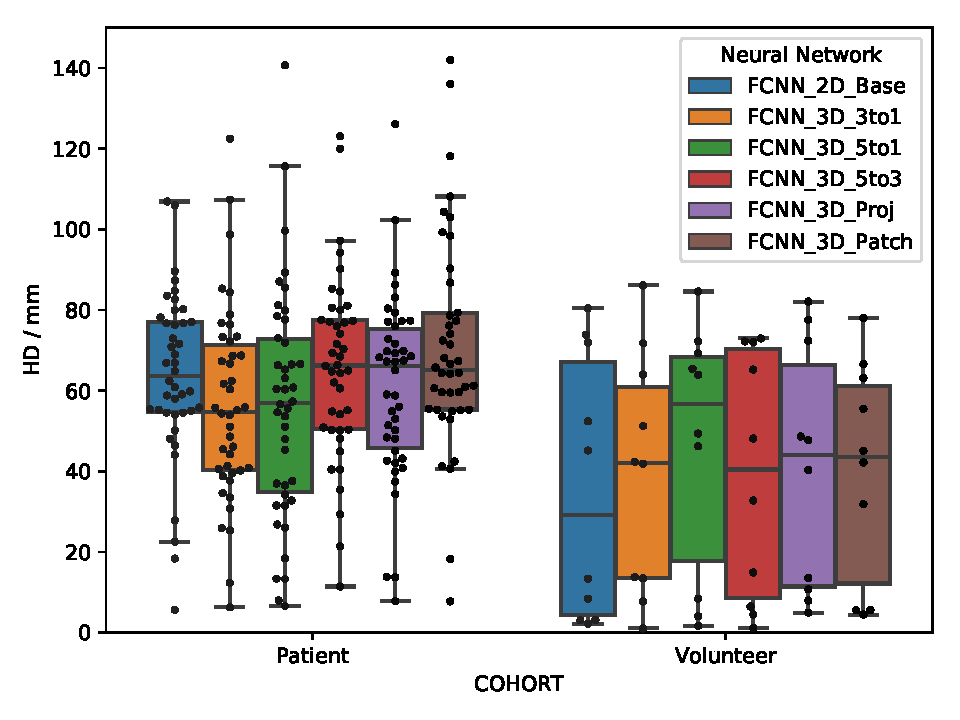
\includegraphics[width=0.8\textwidth]{boxplot_HD}
    \caption[Boxplot for the \acrlong{hd}.]{Boxplot for the \acrlong{hd}.}
    \label{fig:results_boxplot_hd}
\end{figure}

\begin{figure}[htbp]	
	\centering
	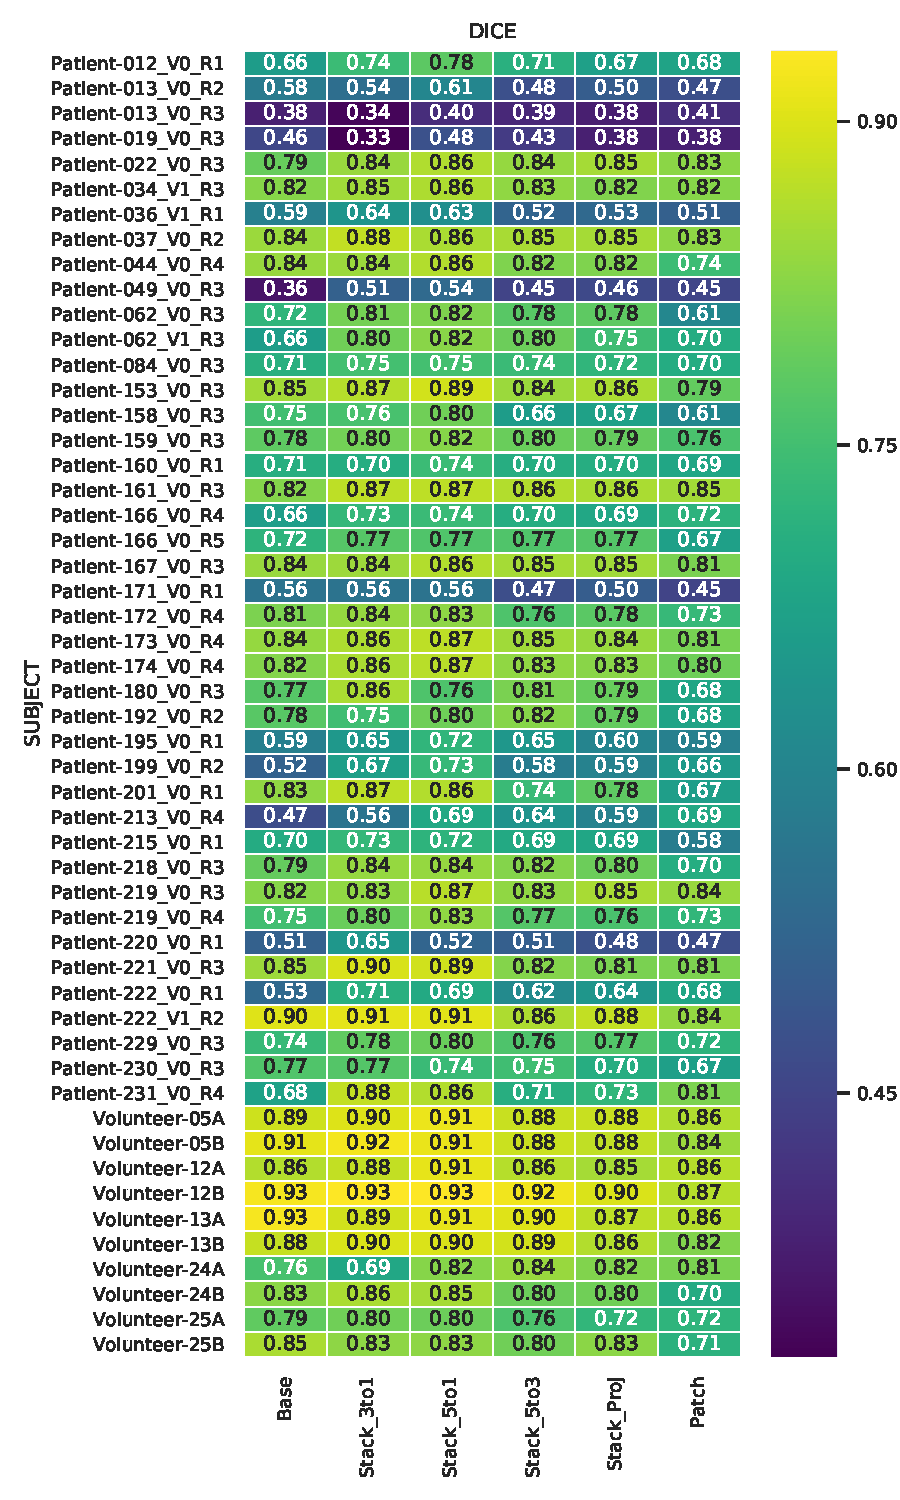
\includegraphics[width=\textwidth]{heat_dice}
    \caption[Heatmap for the \acrlong{dice}.]{Heatmap for the \acrlong{dice}.}
    \label{fig:results_heat_dice}
\end{figure}

\section{Experiment 3: Post-processing} % ===========================================================================

\begin{sidewaystable}[htbp]
   \centering
   \caption[Segmentation Evaluation Metrics for the different Architectures]{}
   \begin{tabular}{l*{7}{l}}
      \toprule
      Cohort	& Network	& Post-processing	& DICE				& VS				& AVD				& HD95				& HD				\\
      			&					&					&					&					& (mm)				& (mm)				& (mm)				\\
      \midrule
      Patient   & 2D\_Base 	& None & $0.705 \pm 0.137$ & $\mathbf{0.883 \pm 0.097}$ & $2.835 \pm 2.655$ & $16.285 \pm 16.896$ & $62.630 \pm 21.803$ \\
                &                	& Volumes only  & $0.711 \pm 0.145$ & $0.867 \pm 0.125$ & $3.431 \pm 4.236$ & $20.364 \pm 20.125$ & $50.726 \pm 21.318$ \\
                &                	& Joint volumes & $\mathbf{0.722 \pm 0.136}$ & $0.873 \pm 0.125$ & $\mathbf{1.705 \pm 1.768}$ & $\mathbf{11.812 \pm 12.785}$& $\mathbf{32.159 \pm 20.178}$ \\
      \midrule
      Patient   & 3D\_5to1 	& None & $0.765 \pm 0.123$ & $0.898 \pm 0.110$ & $2.001 \pm 2.401$ & $12.418 \pm 19.104$ & $56.304 \pm 28.746$ \\
                &                	& Volumes only  & $0.772 \pm 0.120$ & $0.899 \pm 0.119$ & $1.871 \pm 2.534$ & $11.481 \pm 16.706$ & $40.531 \pm 23.941$ \\
                &                	& Joint volumes      & $\mathbf{0.779 \pm 0.123}$ & $\mathbf{0.905 \pm 0.117}$ & $\mathbf{1.106 \pm 1.670}$ & $\mathbf{6.688  \pm 10.332}$ & $\mathbf{28.981 \pm 19.820}$ \\
      \midrule
      Volunteer & 2D\_Base 	& None & $0.861 \pm 0.057$ & $0.921 \pm 0.056$ & $0.643 \pm 0.866$ & $1.644  \pm 2.321 $ & $35.380 \pm 32.720$ \\
                &                	& Volumes only  & $0.862 \pm 0.057$ & $0.924 \pm 0.056$ & $0.608 \pm 0.833$ & $2.311  \pm 4.508 $ & $32.943 \pm 30.360$ \\
                &                	& Joint volumes      & $\mathbf{0.868 \pm 0.050}$ & $\mathbf{0.929 \pm 0.056}$ & $\mathbf{0.197 \pm 0.173}$ & $\mathbf{1.230  \pm 1.255}$ & $\mathbf{7.894  \pm 5.844}$ \\
      \midrule
      Volunteer & 3D\_5to1 	& None & $0.884 \pm 0.046$ & $0.927 \pm 0.051$ & $0.473 \pm 0.399$ & $1.140  \pm 1.344 $ & $46.547 \pm 32.724$ \\
                &                	& Volumes only  & $0.883 \pm 0.046$ & $0.933 \pm 0.049$ & $0.349 \pm 0.224$ & $1.357  \pm 1.454 $ & $32.552 \pm 28.627$ \\
                &                	& Joint volumes      & $\mathbf{0.894 \pm 0.042}$ & $\mathbf{0.942 \pm 0.050}$ & $\mathbf{0.102 \pm 0.060}$ & $\mathbf{0.655  \pm 0.355}$ & $\mathbf{5.177  \pm 2.088}$ \\
      \bottomrule
   \end{tabular}
   \label{tab:results_pp}
\end{sidewaystable}

\begin{figure}[htbp]
	\centering
	\subfloat[]
	{
		\label{fig:subfig:pp_boxplot_base_dice}
		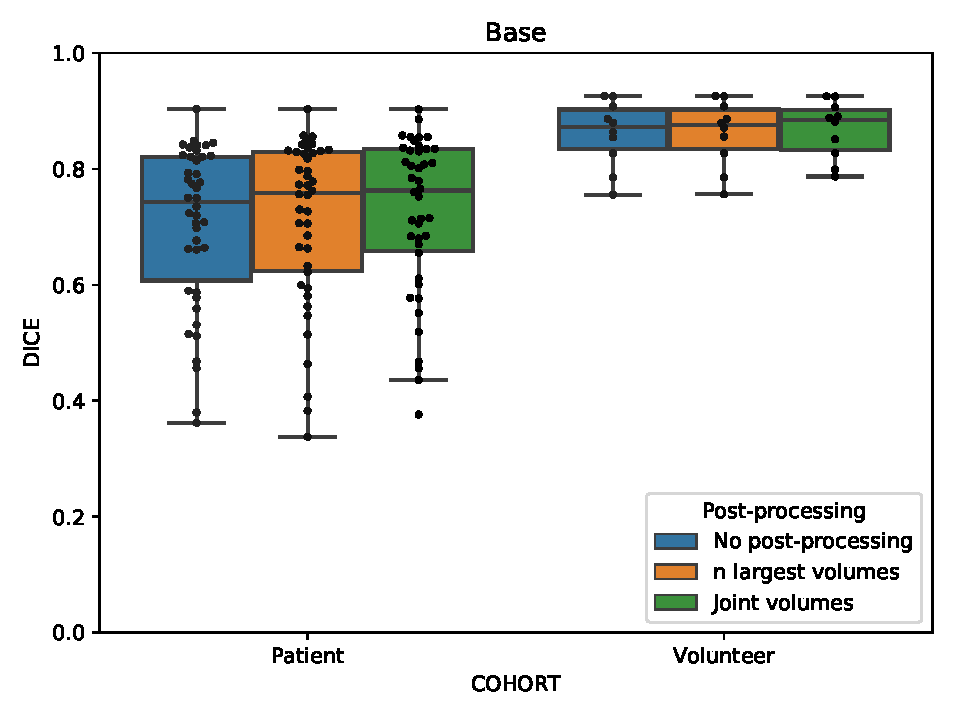
\includegraphics[width=0.7\textwidth]{pp_boxplot_base_DICE}
	}
	\hfill
	\subfloat[]
	{
		\label{fig:subfig:pp_boxplot_5to1_dice}
		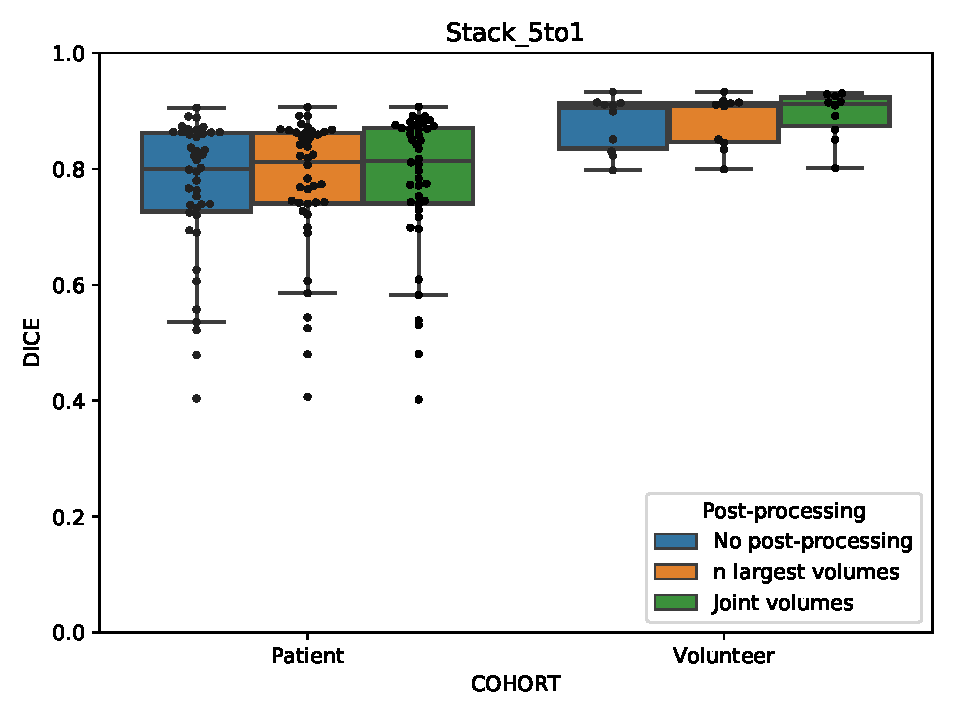
\includegraphics[width=0.7\textwidth]{pp_boxplot_5to1_DICE}
	}
	\caption[Post-processing impact on DICE]{}
	\label{fig:pp_boxplots_dice}  
\end{figure}

\begin{figure}[htbp]
	\centering
	\subfloat[]
	{
		\label{fig:subfig:pp_boxplot_base_vs}
		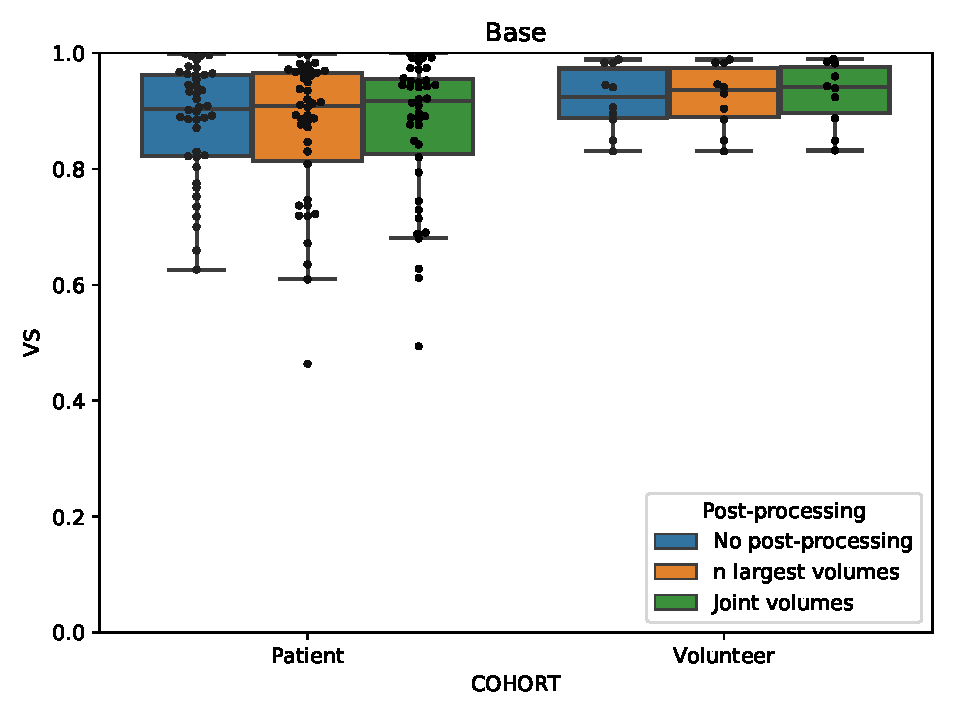
\includegraphics[width=0.7\textwidth]{pp_boxplot_base_VS}
	}
	\hfill
	\subfloat[]
	{
		\label{fig:subfig:pp_boxplot_5to1_vs}
		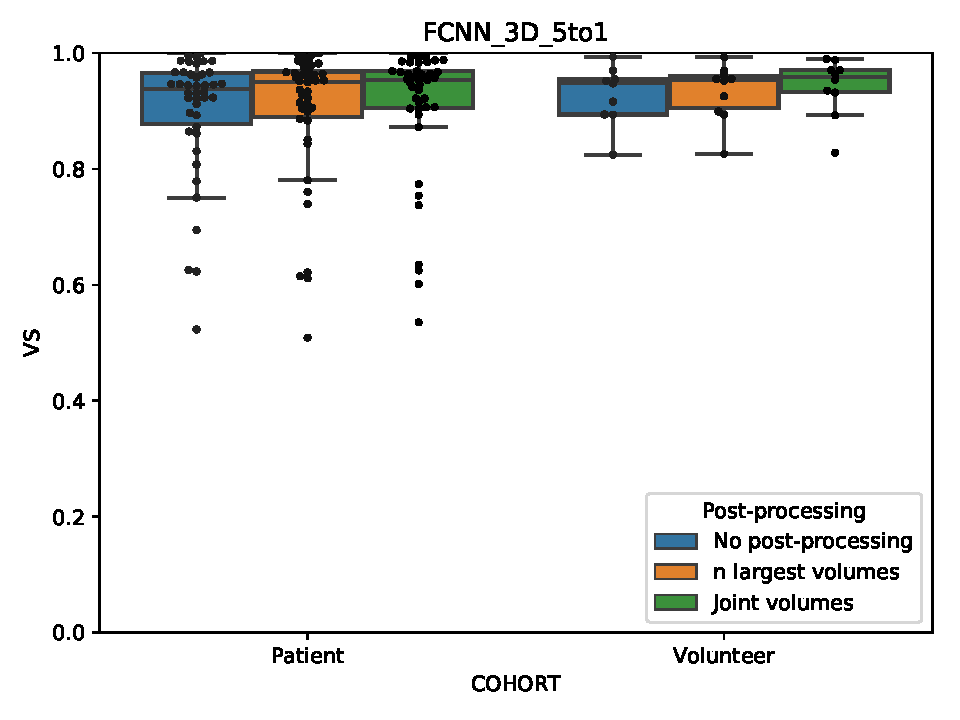
\includegraphics[width=0.7\textwidth]{pp_boxplot_5to1_VS}
	}
	\caption[Post-processing impact on VS]{}
	\label{fig:pp_boxplots_vs}  
\end{figure}

\begin{figure}[htbp]
	\centering
	\subfloat[]
	{
		\label{fig:subfig:pp_boxplot_base_avd}
		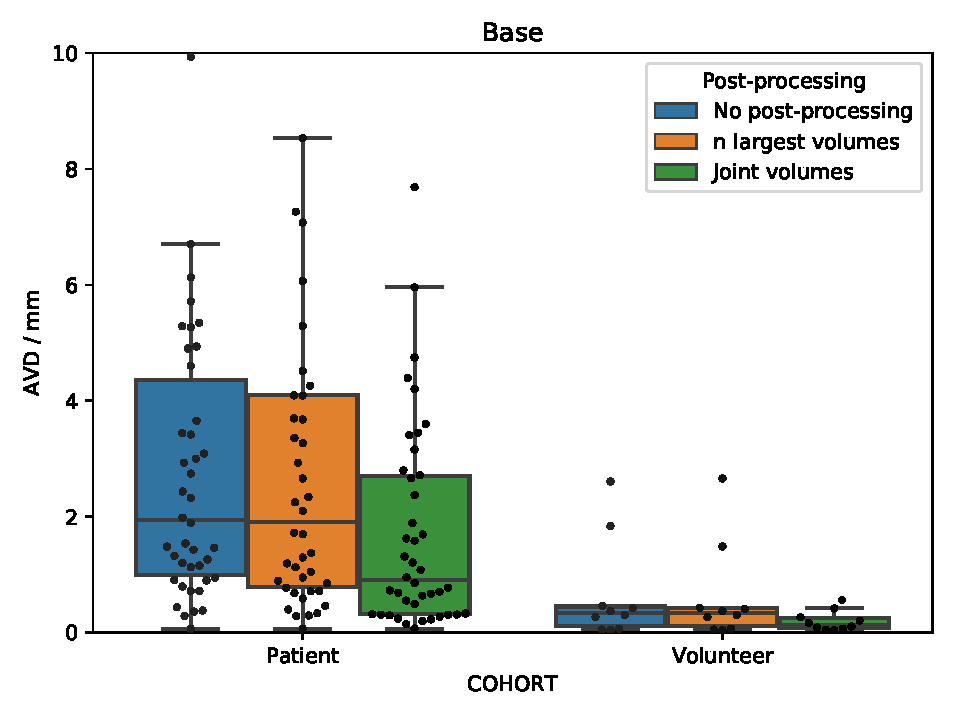
\includegraphics[width=0.7\textwidth]{pp_boxplot_base_AVD}
	}
	\hfill
	\subfloat[]
	{
		\label{fig:subfig:pp_boxplot_5to1_avd}
		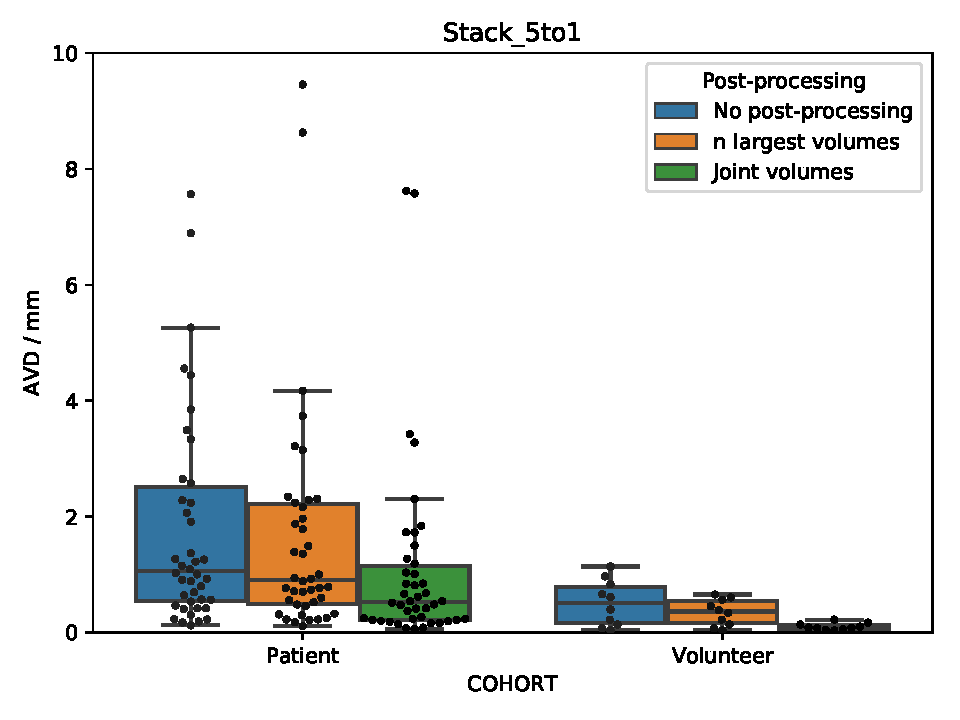
\includegraphics[width=0.7\textwidth]{pp_boxplot_5to1_AVD}
	}
	\caption[Post-processing impact on AVD]{}
	\label{fig:pp_boxplots_avd}  
\end{figure}

\begin{figure}[htbp]
	\centering
	\subfloat[]
	{
		\label{fig:subfig:pp_boxplot_base_hd95}
		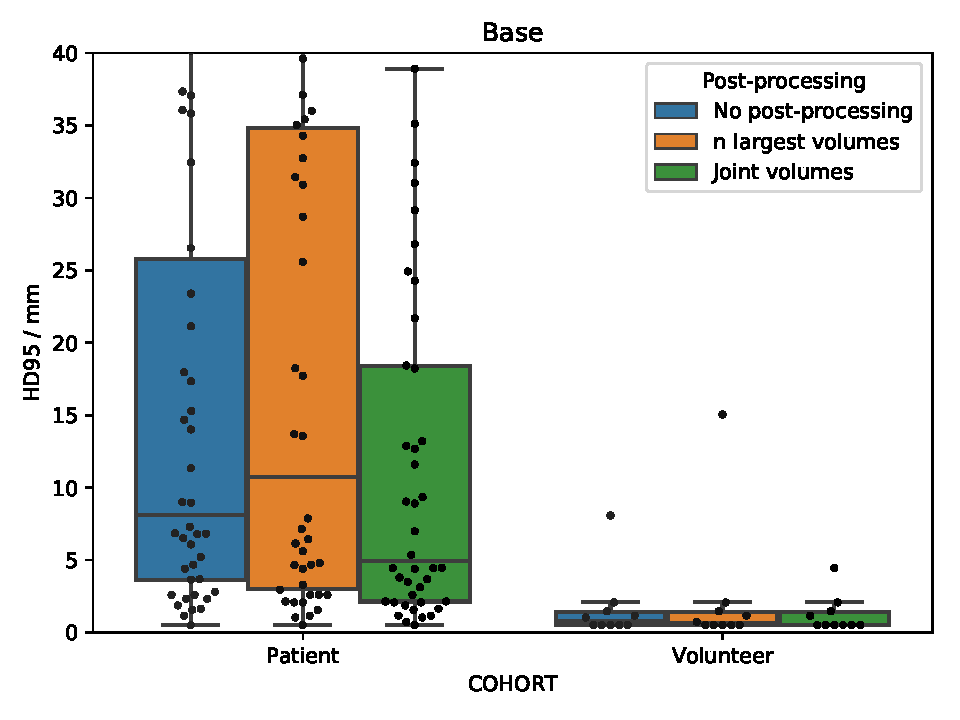
\includegraphics[width=0.7\textwidth]{pp_boxplot_base_HD95}
	}
	\hfill
	\subfloat[]
	{
		\label{fig:subfig:pp_boxplot_5to1_hd95}
		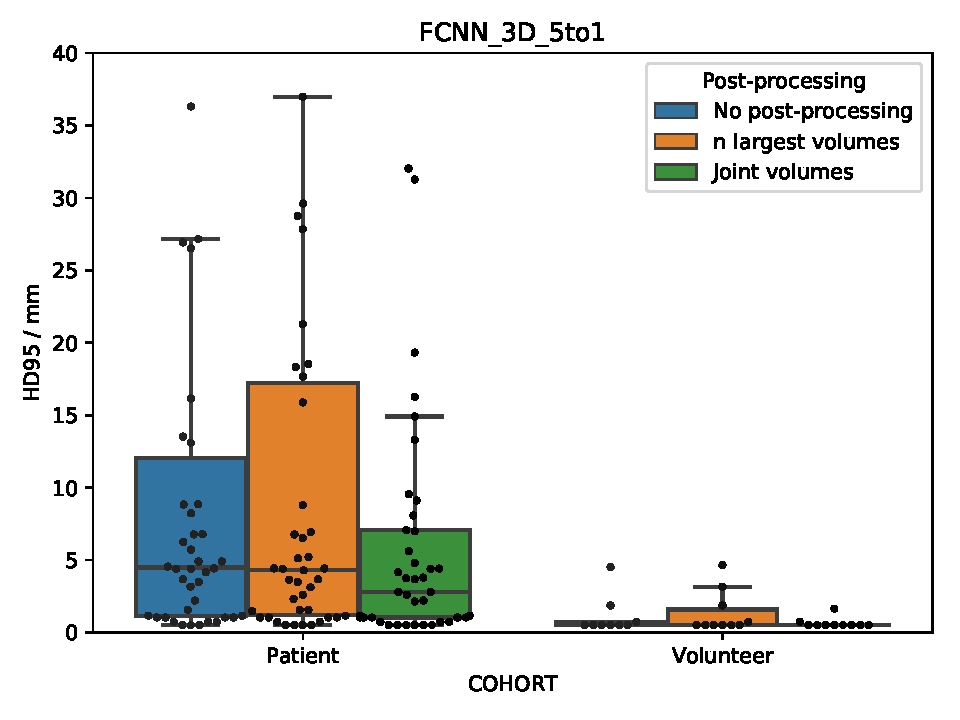
\includegraphics[width=0.7\textwidth]{pp_boxplot_5to1_HD95}
	}
	\caption[Post-processing impact on HD95]{}
	\label{fig:pp_boxplots_hd95}  
\end{figure}

\begin{figure}[htbp]
	\centering
	\subfloat[]
	{
		\label{fig:subfig:pp_boxplot_base_hd}
		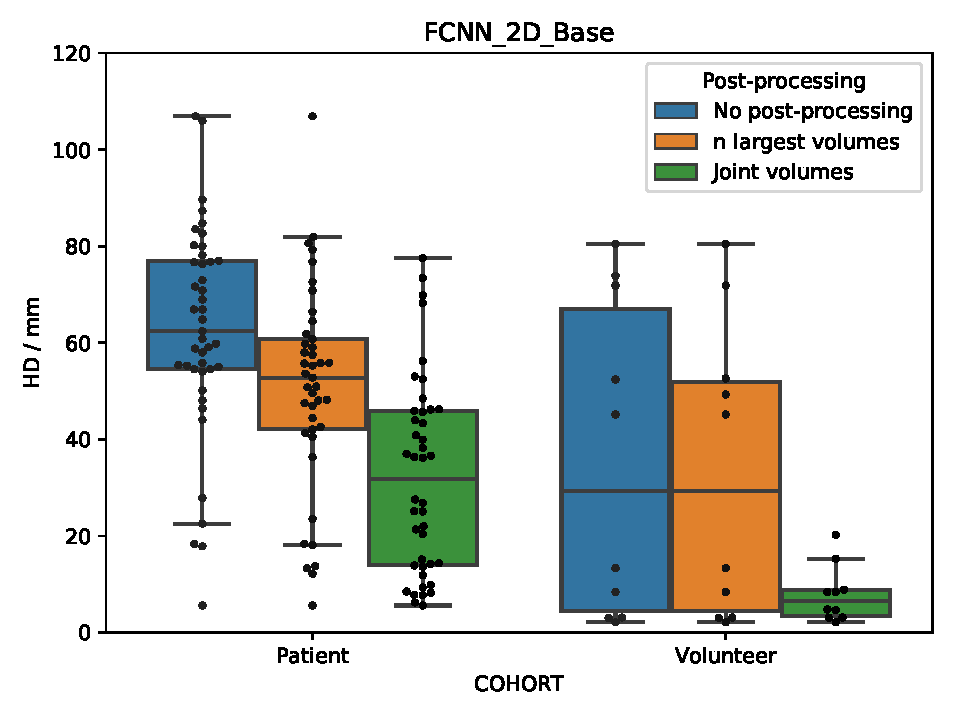
\includegraphics[width=0.7\textwidth]{pp_boxplot_base_HD}
	}
	\hfill
	\subfloat[]
	{
		\label{fig:subfig:pp_boxplot_5to1_hd}
		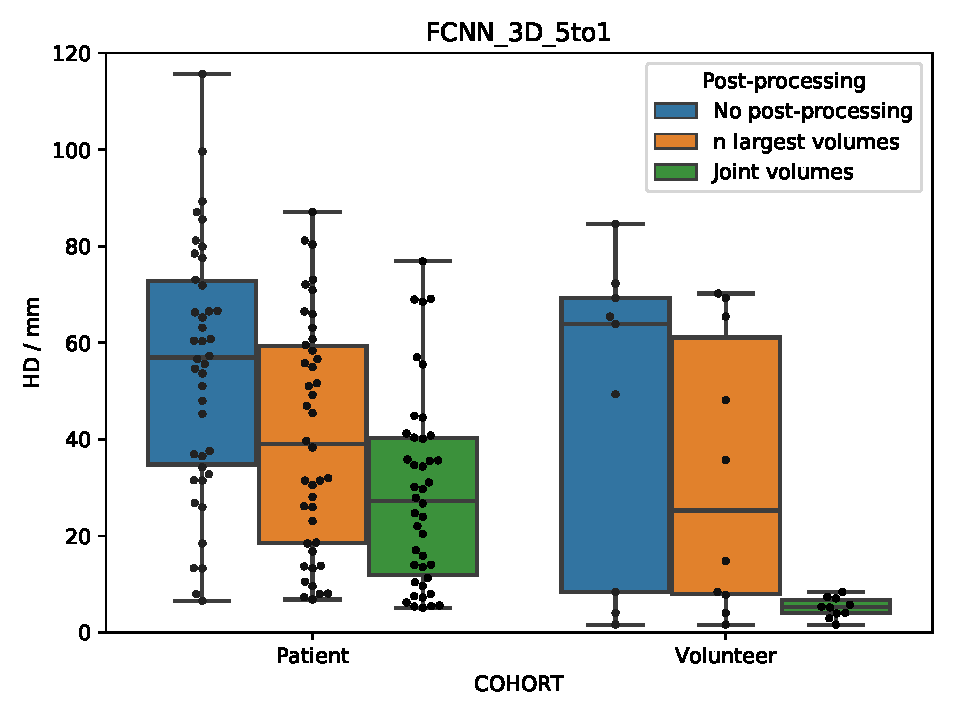
\includegraphics[width=0.7\textwidth]{pp_boxplot_5to1_HD}
	}
	\caption[Post-processing impact on HD]{}
	\label{fig:pp_boxplots_hd}  
\end{figure}

\section{Evaluation: FCNN and Raters} % =============================================================

\begin{figure}[htbp]	
	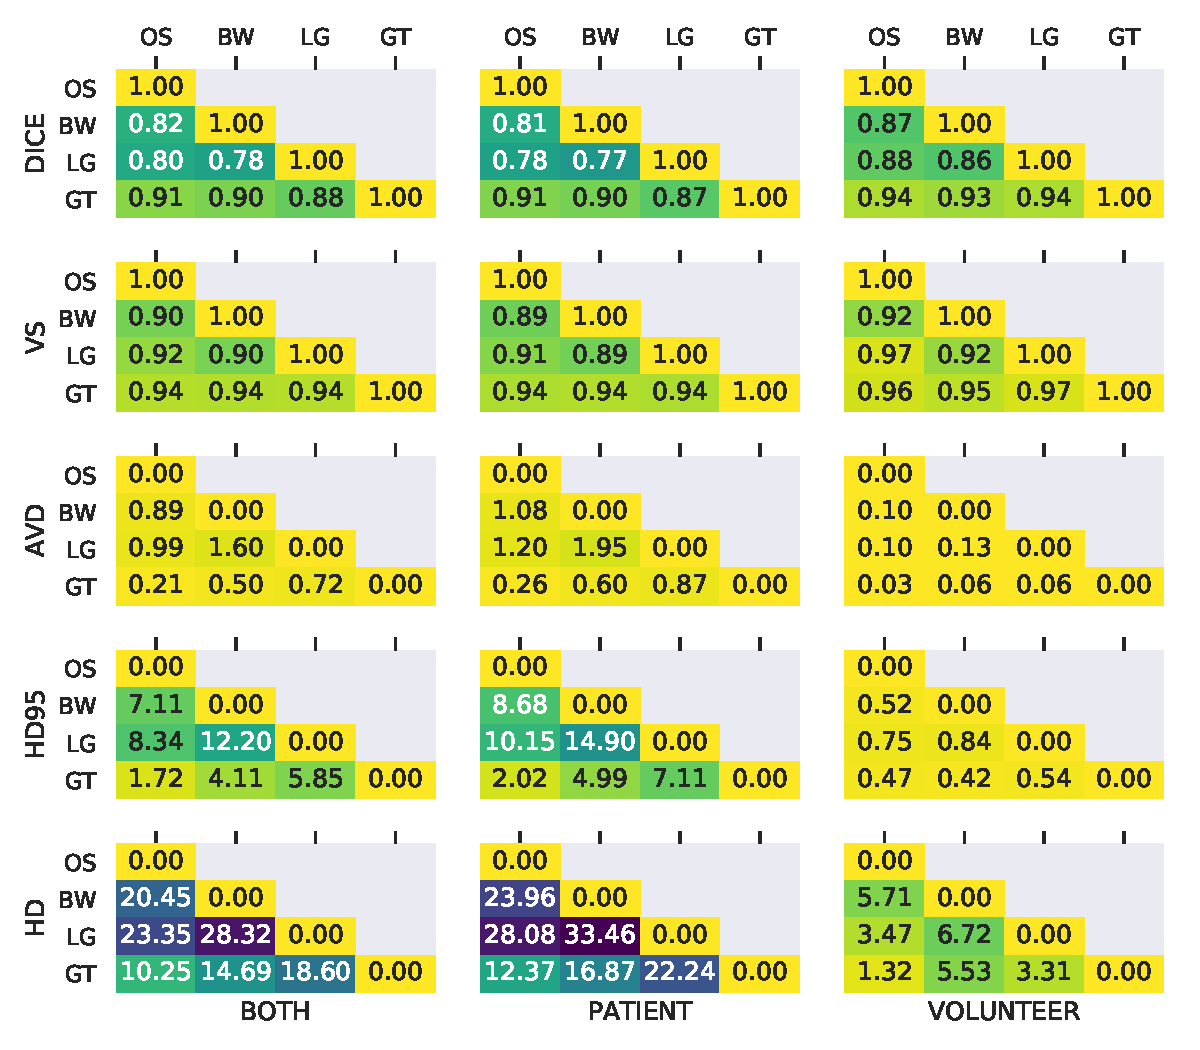
\includegraphics[width=\textwidth]{inter_rater}
    \caption[Inter-Rater Agreement]{Inter-rater agreement for the DICE, VS, AVD, HD95 and HD metrics. Values close to 1.00 for DICE and VS correspond to a high level of agreement between the raters. Conversely, low values for AVD, HD95 and HD imply higher level agreement.}
    \label{fig:inter_rater}
\end{figure}

\chapter{Network Architectures} % =================================================================================

\begin{sidewaystable}[htbp]
   \centering
   \caption[Architecture of FCNN 2D Baseline]{Detailed architecture of the baseline neural network.}
   \begin{tabular}{l*{4}{l}}
      \toprule
      Level	& Layer						& Properties 					& In 									& Out	\\
      		&							&								& $C \times D \times H \times W$		& $C \times D \times H \times W$		\\
      \midrule
      1D	& Conv2D, Dropout, BN, ReLU & K: $3 \times 3$, P1, S1		& $2 \times 1 \times 300 \times 300$	& $32 \times 1 \times 300 \times 300$	\\
      1D	& Conv2D, Dropout, BN, ReLU & K: $3 \times 3$, P1, S1		& $32 \times 1 \times 300 \times 300$	& $32 \times 1 \times 300 \times 300$	\\
      2D	& Max Pooling				& K: $2 \times 2$, P0, S2		& $32 \times 1 \times 300 \times 300$	& $32 \times 1 \times 150 \times 150$	\\
      2D	& Conv2D, Dropout, BN, ReLU & K: $3 \times 3$, P1, S1		& $32 \times 1 \times 150 \times 150$	& $64 \times 1 \times 150 \times 150$	\\
      2D	& Conv2D, Dropout, BN, ReLU & K: $3 \times 3$, P1, S1		& $64 \times 1 \times 150 \times 150$	& $64 \times 1 \times 150 \times 150$	\\
      3D	& Max Pooling				& K: $2 \times 2$, P0, S2		& $64 \times 1 \times 150 \times 150$	& $64 \times 1 \times 75 \times 75$		\\
      3D	& Conv2D, Dropout, BN, ReLU & K: $3 \times 3$, P1, S1		& $64 \times 1 \times 75 \times 75$		& $128 \times 1 \times 75 \times 75$	\\
      3D	& Conv2D, Dropout, BN, ReLU & K: $3 \times 3$, P1, S1		& $128 \times 1 \times 75 \times 75$	& $128 \times 1 \times 75 \times 75$	\\
      4D	& Max Pooling				& K: $2 \times 2$, P0, S2		& $128 \times 1 \times 75 \times 75$	& $128 \times 1 \times 37 \times 37$	\\
      4D	& Conv2D, Dropout, BN, ReLU & K: $3 \times 3$, P1, S1		& $128 \times 1 \times 37 \times 37$	& $256 \times 1 \times 37 \times 37$	\\
      4D	& Conv2D, Dropout, BN, ReLU & K: $3 \times 3$, P1, S1		& $256 \times 1 \times 37 \times 37$	& $256 \times 1 \times 37 \times 37$	\\
      5D	& Max Pooling				& K: $2 \times 2$, P0, S2		& $256 \times 1 \times 37 \times 37$	& $256 \times 1 \times 18 \times 18$	\\
      5D	& Conv2D, Dropout, BN, ReLU & K: $3 \times 3$, P1, S1		& $256 \times 1 \times 18 \times 18$	& $512 \times 1 \times 18 \times 18$	\\
      5D	& Conv2D, Dropout, BN, ReLU & K: $3 \times 3$, P1, S1		& $512 \times 1 \times 18 \times 18$	& $512 \times 1 \times 18 \times 18$	\\
      
      4U	& ConvTranspose2D			& K: $2 \times 2$, P0, S2		& $512 \times 1 \times 18 \times 18$	& $256 \times 1 \times 37 \times 37$	\\
      4U	& Concat Skip Feature Map	&								&										& $512 \times 1 \times 37 \times 37$	\\
      4U	& Conv2D, Dropout, BN, ReLU & K: $3 \times 3$, P1, S1		& $512 \times 1 \times 37 \times 37$	& $256 \times 1 \times 37 \times 37$	\\
      4U	& Conv2D, Dropout, BN, ReLU & K: $3 \times 3$, P1, S1		& $256 \times 1 \times 37 \times 37$	& $256 \times 1 \times 37 \times 37$	\\
      3U	& ConvTranspose2D			& K: $2 \times 2$, P0, S2		& $256 \times 1 \times 37 \times 37$	& $128 \times 1 \times 75 \times 75$	\\
      3U	& Concat Skip Feature Map	&								&										& $256 \times 1 \times 75 \times 75$	\\
      3U	& Conv2D, Dropout, BN, ReLU & K: $3 \times 3$, P1, S1		& $256 \times 1 \times 75 \times 75$	& $128 \times 1 \times 75 \times 75$	\\
      3U	& Conv2D, Dropout, BN, ReLU & K: $3 \times 3$, P1, S1		& $128 \times 1 \times 75 \times 75$	& $128 \times 1 \times 75 \times 75$	\\
      2U	& ConvTranspose2D			& K: $2 \times 2$, P0, S2		& $128 \times 1 \times 75 \times 75$	& $64 \times 1 \times 150 \times 150$	\\
      2U	& Concat Skip Feature Map	&								&										& $128 \times 1 \times 150 \times 150$	\\
      2U	& Conv2D, Dropout, BN, ReLU & K: $3 \times 3$, P1, S1		& $128 \times 1 \times 150 \times 150$	& $64 \times 1 \times 150 \times 150$	\\
      2U	& Conv2D, Dropout, BN, ReLU & K: $3 \times 3$, P1, S1		& $64 \times 1 \times 150 \times 150$	& $64 \times 1 \times 150 \times 150$	\\
      1U	& ConvTranspose2D			& K: $2 \times 2$, P0, S2		& $128 \times 1 \times 150 \times 150$	& $32 \times 1 \times 300 \times 300$	\\
      1U	& Concat Skip Feature Map	&								&										& $64 \times 1 \times 300 \times 300$	\\
      1U	& Conv2D, Dropout, BN, ReLU & K: $3 \times 3$, P1, S1		& $64 \times 1 \times 300 \times 300$	& $32 \times 1 \times 300 \times 300$	\\
      1U	& Conv2D, Dropout, BN, ReLU & K: $3 \times 3$, P1, S1		& $32 \times 1 \times 300 \times 300$	& $32 \times 1 \times 300 \times 300$	\\
      
      Out	& Conv2D					& K: $1 \times 1$, P0, S1		& $32 \times 1 \times 300 \times 300$	& $1 \times 1 \times 300 \times 300$	\\
      \bottomrule
   \end{tabular}
   \label{tab:architecture_fcnn_base}
\end{sidewaystable}

\begin{sidewaystable}[htbp]
   \centering
   \caption[Architecture of FCNN 3D Volumetric]{Detailed architecture of the volumetric neural network. $I$, $O$ correspond to the chosen number of input and output slices, respectively. The following combinations have been trained: $I = 3$, $O = 1$ (3-to-1), $I = 5$, $O = 1$ (5-to-1), $I = 5$, $O = 3$ (5-to-3).}
   \begin{tabular}{l*{4}{l}}
      \toprule
      Level	& Layer				& Properties 					& In							& Out									\\
      &							&								& $C \times D \times H \times W$& $C \times D \times H \times W$		\\
      \midrule
      1D	& Conv3D, Dropout, BN, ReLU & K: $1 \times 3 \times 3$, P(0, 1, 1), S1	& $2 \times I \times 300 \times 300$	& $32 \times I \times 300 \times 300$	\\
      1D	& Conv3D, Dropout, BN, ReLU & K: $3 \times 3 \times 3$, P1, S1			& $32 \times I \times 300 \times 300$	& $32 \times I \times 300 \times 300$	\\
      2D	& Max Pooling				& K: $1 \times 2 \times 2$, P0, S(1, 2, 2)	& $32 \times I \times 300 \times 300$	& $32 \times I \times 150 \times 150$	\\
      2D	& Conv3D, Dropout, BN, ReLU & K: $1 \times 3 \times 3$, P(0, 1, 1), S1	& $32 \times I \times 150 \times 150$	& $64 \times I \times 150 \times 150$	\\
      2D	& Conv3D, Dropout, BN, ReLU & K: $3 \times 3 \times 3$, P1, S1			& $64 \times I \times 150 \times 150$	& $64 \times I \times 150 \times 150$	\\
      3D	& Max Pooling				& K: $1 \times 2 \times 2$, P0, S(1, 2, 2)	& $64 \times I \times 150 \times 150$	& $64 \times I \times 75 \times 75$		\\
      3D	& Conv3D, Dropout, BN, ReLU & K: $1 \times 3 \times 3$, P(0, 1, 1), S1	& $64 \times I \times 75 \times 75$		& $128 \times I \times 75 \times 75$	\\
      3D	& Conv3D, Dropout, BN, ReLU & K: $3 \times 3 \times 3$, P1, S1			& $128 \times I \times 75 \times 75$	& $128 \times I \times 75 \times 75$	\\
      4D	& Max Pooling				& K: $1 \times 2 \times 2$, P0, S(1, 2, 2)	& $128 \times I \times 75 \times 75$	& $128 \times I \times 37 \times 37$	\\
      4D	& Conv3D, Dropout, BN, ReLU & K: $1 \times 3 \times 3$, P(0, 1, 1), S1	& $128 \times I \times 37 \times 37$	& $256 \times I \times 37 \times 37$	\\
      4D	& Conv3D, Dropout, BN, ReLU & K: $3 \times 3 \times 3$, P1, S1			& $256 \times I \times 37 \times 37$	& $256 \times I \times 37 \times 37$	\\
      5D	& Max Pooling				& K: $1 \times 2 \times 2$, P0, S(1, 2, 2)	& $256 \times I \times 37 \times 37$	& $256 \times I \times 18 \times 18$	\\
      5D	& Conv3D, Dropout, BN, ReLU & K: $1 \times 3 \times 3$, P(0, 1, 1), S1	& $256 \times I \times 18 \times 18$	& $512 \times I \times 18 \times 18$	\\
      5D	& Conv3D, Dropout, BN, ReLU & K: $3 \times 3 \times 3$, P1, S1			& $512 \times I \times 18 \times 18$	& $512 \times I \times 18 \times 18$	\\
      
      4U	& ConvTranspose3D			& K: $1 \times 2 \times 2$, P0, S(1, 2, 2)	& $512 \times I \times 18 \times 18$	& $256 \times I \times 37 \times 37$	\\
      4U	& Concat Skip Feature Map	&											&										& $512 \times I \times 37 \times 37$	\\
      4U	& Conv3D, Dropout, BN, ReLU & K: $1 \times 3 \times 3$, P(0, 1, 1), S1	& $512 \times I \times 37 \times 37$	& $256 \times I \times 37 \times 37$	\\
      4U	& Conv3D, Dropout, BN, ReLU & K: $3 \times 3 \times 3$, P1, S1			& $256 \times I \times 37 \times 37$	& $256 \times I \times 37 \times 37$	\\
      3U	& ConvTranspose3D			& K: $1 \times 2 \times 2$, P0, S(1, 2, 2)	& $256 \times I \times 37 \times 37$	& $128 \times I \times 75 \times 75$	\\
      3U	& Concat Skip Feature Map	&											&										& $256 \times I \times 75 \times 75$	\\
      3U	& Conv3D, Dropout, BN, ReLU & K: $1 \times 3 \times 3$, P(0, 1, 1), S1	& $256 \times I \times 75 \times 75$	& $128 \times I \times 75 \times 75$	\\
      3U	& Conv3D, Dropout, BN, ReLU & K: $3 \times 3 \times 3$, P1, S1			& $128 \times I \times 75 \times 75$	& $128 \times I \times 75 \times 75$	\\
      2U	& ConvTranspose3D			& K: $1 \times 2 \times 2$, P0, S(1, 2, 2)	& $128 \times I \times 75 \times 75$	& $64 \times I \times 150 \times 150$	\\
      2U	& Concat Skip Feature Map	&											&										& $128 \times I \times 150 \times 150$	\\
      2U	& Conv3D, Dropout, BN, ReLU & K: $1 \times 3 \times 3$, P(0, 1, 1), S1	& $128 \times I \times 150 \times 150$	& $64 \times I \times 150 \times 150$	\\
      2U	& Conv3D, Dropout, BN, ReLU & K: $3 \times 3 \times 3$, P1, S1			& $64 \times I \times 150 \times 150$	& $64 \times I \times 150 \times 150$	\\
      1U	& ConvTranspose2D			& K: $1 \times 2 \times 2$, P0, S(1, 2, 2)	& $128 \times I \times 150 \times 150$	& $32 \times I \times 300 \times 300$	\\
      1U	& Concat Skip Feature Map	&											&										& $64 \times I \times 300 \times 300$	\\
      1U	& Conv3D, Dropout, BN, ReLU & K: $1 \times 3 \times 3$, P(0, 1, 1), S1	& $64 \times I \times 300 \times 300$	& $32 \times I \times 300 \times 300$	\\
      1U	& Conv3D, Dropout, BN, ReLU & K: $3 \times 3 \times 3$, P1, S1			& $32 \times I \times 300 \times 300$	& $32 \times I \times 300 \times 300$	\\
      			
      Out	& Conv3D					& K: $I \times 1 \times 1$, P0, S1			& $32 \times I \times 300 \times 300$	& $1 \times O \times 300 \times 300$	\\
      \bottomrule
   \end{tabular}
   \label{tab:architecture_fcnn_volumetric}
\end{sidewaystable}

\begin{sidewaystable}[htbp]
   \centering
   \caption[Architecture of FCNN 3D Patches]{Detailed architecture of the patch-based neural network.}
   \begin{tabular}{l*{4}{l}}
      \toprule
      Level	& Layer						& Properties 					& In							& Out									\\
      		&							&								& $C \times D \times H \times W$& $C \times D \times H \times W$		\\
      \midrule
      1D	& Conv2D, Dropout, BN, ReLU & K: $3 \times 3 \times 3$, P1, S1			& $2 \times 12 \times 128 \times 128$	&	$32 \times 12 \times 128 \times 128$	\\
      1D	& Conv2D, Dropout, BN, ReLU & K: $3 \times 3 \times 3$, P1, S1			& $32 \times 12 \times 128 \times 128$	&	$32 \times 12 \times 128 \times 128$	\\
      2D	& Max Pooling				& K: $1 \times 2 \times 2$, P0, S(1, 2, 2)	& $32 \times 12 \times 128 \times 128$	&	$32 \times 12 \times 64 \times 64$	\\
      2D	& Conv2D, Dropout, BN, ReLU & K: $3 \times 3 \times 3$, P1, S1			& $32 \times 12 \times 64 \times 64$	&	$64 \times 12 \times 64 \times 64$	\\
      2D	& Conv2D, Dropout, BN, ReLU & K: $3 \times 3 \times 3$, P1, S1			& $64 \times 12 \times 64 \times 64$	& 	$64 \times 12 \times 64 \times 64$	\\
      3D	& Max Pooling				& K: $1 \times 2 \times 2$, P0, S(1, 2, 2)	& $64 \times 12 \times 64 \times 64$	& 	$64 \times 12 \times 32 \times 32$		\\
      3D	& Conv2D, Dropout, BN, ReLU & K: $3 \times 3 \times 3$, P1, S1			& $64 \times 12 \times 32 \times 32$	&	$128 \times 12 \times 32 \times 32$	\\
      3D	& Conv2D, Dropout, BN, ReLU & K: $3 \times 3 \times 3$, P1, S1			& $128 \times 12 \times 32 \times 32$	&	$128 \times 12 \times 32 \times 32$	\\
      4D	& Max Pooling				& K: $1 \times 2 \times 2$, P0, S(1, 2, 2)	& $128 \times 12 \times 32 \times 32$	&	$128 \times 12 \times 16 \times 16$	\\
      4D	& Conv2D, Dropout, BN, ReLU & K: $3 \times 3 \times 3$, P1, S1			& $128 \times 12 \times 16 \times 16$	&	$256 \times 12 \times 16 \times 16$	\\
      4D	& Conv2D, Dropout, BN, ReLU & K: $3 \times 3 \times 3$, P1, S1			& $256 \times 12 \times 16 \times 16$	&	$256 \times 12 \times 16 \times 16$	\\
      
      3U	& ConvTranspose2D			& K: $1 \times 2 \times 2$, P0, S(1, 2, 2)	& $256 \times 12 \times 16 \times 16$	& $128 \times 12 \times 32 \times 32$	\\
      3U	& Concat Skip Feature Map	&								&													& $256 \times 12 \times 32 \times 32$	\\
      3U	& Conv2D, Dropout, BN, ReLU & K: $3 \times 3 \times 3 \times 3$, P1, S1	& $256 \times 12 \times 32 \times 32$	& $128 \times 12 \times 32 \times 32$	\\
      3U	& Conv2D, Dropout, BN, ReLU & K: $3 \times 3 \times 3 \times 3$, P1, S1	& $128 \times 12 \times 32 \times 32$	& $128 \times 12 \times 32 \times 32$	\\
      2U	& ConvTranspose2D			& K: $1 \times 2 \times 2$, P0, S(1, 2, 2)	& $128 \times 12 \times 32 \times 32$	& $64 \times 12 \times 64 \times 64$	\\
      2U	& Concat Skip Feature Map	&								&													& $128 \times 12 \times 64 \times 64$	\\
      2U	& Conv2D, Dropout, BN, ReLU & K: $3 \times 3 \times 3 \times 3$, P1, S1	& $128 \times 12 \times 64 \times 64$	& $64 \times 12 \times 64 \times 64$	\\
      2U	& Conv2D, Dropout, BN, ReLU & K: $3 \times 3 \times 3 \times 3$, P1, S1	& $64 \times 12 \times 64 \times 64$	& $64 \times 12 \times 64 \times 64$	\\
      1U	& ConvTranspose2D			& K: $1 \times 2 \times 2$, P0, S(1, 2, 2)	& $128 \times 12 \times 64 \times 64$	& $32 \times 12 \times 128 \times 128$	\\
      1U	& Concat Skip Feature Map	&								&													& $64 \times 12 \times 128 \times 128$	\\
      1U	& Conv2D, Dropout, BN, ReLU & K: $3 \times 3 \times 3 \times 3$, P1, S1	& $64 \times 12 \times 128 \times 128$	& $32 \times 12 \times 128 \times 128$	\\
      1U	& Conv2D, Dropout, BN, ReLU & K: $3 \times 3 \times 3 \times 3$, P1, S1	& $32 \times 12 \times 128 \times 128$	& $32 \times 12 \times 128 \times 128$	\\
      
      Out	& Conv2D					& K: $1 \times 1 \times 1$, P0, S1			& $32 \times 12 \times 128 \times 128$	& $1 \times 12 \times 128 \times 128$	\\
      \bottomrule
   \end{tabular}
   \label{tab:architecture_fcnn_patches}
\end{sidewaystable}

\chapter{Additional Tables} % =====================================================================================

\begin{table}[htbp]
   \centering
   \caption{Assignment of subjects to the different folds for the four-fold cross-validation.}
   \begin{tabular}{p{3cm}l}
      \toprule
      \textbf{Fold-0} & $n = 13$ \\      
      Subject & Cohort \\
      \midrule
      05B           & Volunteer \\
      25A           & Volunteer \\
      012\_V0\_R1  & Patient   \\
      037\_V0\_R2  & Patient   \\
      044\_V0\_R4  & Patient   \\
      084\_V0\_R3  & Patient   \\
      159\_V0\_R3 & Patient   \\
      173\_V0\_R4 & Patient   \\
      174\_V0\_R4 & Patient   \\
      199\_V0\_R2 & Patient   \\
      221\_V0\_R3 & Patient   \\
      229\_V0\_R3 & Patient   \\
      231\_V0\_R4 & Patient   \\
      \bottomrule
   \end{tabular}
   \begin{tabular}{p{3cm}l}      
      \toprule
      \textbf{Fold-1} & $n = 13$ \\
      Subject & Cohort \\
      \midrule
      05A           & Volunteer \\
      12A           & Volunteer \\
      013\_V0\_R3  & Patient   \\
      022\_V0\_R3  & Patient   \\
      034\_V1\_R3  & Patient   \\
      161\_V0\_R3 & Patient   \\
      166\_V0\_R4 & Patient   \\
      167\_V0\_R3 & Patient   \\
      192\_V0\_R2 & Patient   \\
      213\_V0\_R4 & Patient   \\
      218\_V0\_R3 & Patient   \\
      220\_V0\_R1 & Patient   \\
      222\_V0\_R1 & Patient   \\      
      \bottomrule
   \end{tabular}
   \begin{tabular}{p{3cm}l}
      \textbf{Fold-2} & $n = 13$ \\
      Subject & Cohort \\
      \midrule
      12B           & Volunteer \\
      13A           & Volunteer \\
      24A           & Volunteer \\
      049\_V0\_R3  & Patient   \\
      062\_V0\_R3  & Patient   \\
      153\_V0\_R3 & Patient   \\
      158\_V0\_R3 & Patient   \\
      160\_V0\_R1 & Patient   \\
      166\_V0\_R5 & Patient   \\
      171\_V0\_R1 & Patient   \\
      201\_V0\_R1 & Patient   \\
      219\_V0\_R4 & Patient   \\
      222\_V1\_R2 & Patient   \\      
      \bottomrule
   \end{tabular}
   \begin{tabular}{p{3cm}l}
      \textbf{Fold-3} & $n = 13$ \\
      Subject & Cohort \\
      \midrule
      13B           & Volunteer \\
      24B           & Volunteer \\
      25B           & Volunteer \\
      013\_V0\_R2  & Patient   \\
      019\_V0\_R3  & Patient   \\
      036\_V1\_R1  & Patient   \\
      062\_V1\_R3  & Patient   \\
      172\_V0\_R4 & Patient   \\
      180\_V0\_R3 & Patient   \\
      195\_V0\_R1 & Patient   \\      
      215\_V0\_R1 & Patient   \\
      219\_V0\_R3 & Patient   \\
      230\_V0\_R3 & Patient   \\      
      \bottomrule
   \end{tabular}
   \label{tab:fold_assignment}
\end{table}

\begin{sidewaystable}[htbp]
   \centering
   \caption[Hyperparameters]{The used hyperparemeters for the different network architectures we trained.}
   \begin{tabular}{l*{7}{l}}
      \toprule
      Neural Network & Epochs	& Batchsize & Learning Rate & Steps & Momentum & In & Out \\
      		&			&	&	&	&	& $D \times H \times W$	&  $D \times H \times W$	\\
      \midrule
      FCNN\_2D\_Base	& 150	& 32	& 0.001	& 100, 125 & 0.99	& $1 \times 300 \times 300$	& $1 \times 300 \times 300$ \\
      \midrule
      FCNN\_3D\_3to1 & 200	& 8	& 0.0001 & 180, 190 & 0.99 & $3 \times 300 \times 300$ & $1 \times 300 \times 300$ \\
      FCNN\_3D\_5to1 	& 200	& 8	& 0.0001 & 180, 190 & 0.99 & $5 \times 300 \times 300$ & $1 \times 300 \times 300$ \\
      FCNN\_3D\_5to3 	& 200	& 6	& 0.0001 & 180, 190 & 0.99 & $5 \times 300 \times 300$ & $3 \times 300 \times 300$ \\
      FCNN\_3D\_Patch & 500	& 16	& 0.0001 & 400, 450 & 0.99 & $12 \times 128 \times 128$ & $12 \times 128 \times 128$ \\
      FCNN\_3D\_Proj & 200	& 6	& 0.0001 & 180, 190 & 0.99 & $5 \times 300 \times 300$ & $3 \times 300 \times 300$ \\
      \bottomrule
   \end{tabular}
   \label{tab:hyperparameters}
\end{sidewaystable}




